\documentclass{beamer}
% AnnArbor  Antibes  Bergen  Berkeley  Berlin  Boadilla  CambridgeUS  Copenhagen  Darmstadt  Dresden  Frankfurt  Goettingen  Hannover  Ilmenau  JuanLesPins  Luebeck  Madrid  Malmoe  Marburg  Montpellier  PaloAlto  Pittsburgh  Rochester  Singapore  Szeged  Warsaw  boxes  default 
\mode<presentation>
{
  \usetheme{Antibes}
  \setbeamercovered{transparent}
}

\usepackage[english]{babel}
\usepackage{times}
\usepackage{graphicx}           
\usepackage{xeCJK}       
\usepackage{fontspec}
\setsansfont{SimSun}

\title[Assignment 4] 
{EAS Integration Project Presentation}

\subtitle
{Perspectives and Facts on How to Design and Implement EAS Integration Project}

\author[Author] 
{吴继鹏}

\institute[Universities of Somewhere and Elsewhere] 
{
  Software Institute\\
  Nanjing University
}

\date[Integration 2014]
{Integration, 2014}

\subject{Theoretical Computer Science}
\AtBeginSubsection[]
{
  \begin{frame}<beamer>{Outline}
    \tableofcontents[currentsection,currentsubsection]
  \end{frame}
}
\begin{document}

\begin{frame}
  \titlepage
\end{frame}

\begin{frame}{Outline}
  \tableofcontents
\end{frame}

\section{Abstract}
\begin{frame}
\begin{enumerate}
\item 展示我们的功能实现情况。
\item 展示我们的设计思路。
\item 展示其他抽象层次的观点。
\end{enumerate}
\end{frame}


\section{Facts about Implementations}
\begin{frame}
  我们做了哪些?
\begin{enumerate}
\item 实现了3个教务系统服务器和1个集成服务器。\pause
\item 每个教务系统服务器都提供一下服务:\pause
  \begin{enumerate}
  \item 专门监听其他服务器的HttpRequest的服务:\pause
    \begin{enumerate}
    \item CourseProvider: 从数据库里提取课程数据,转化为XML,然后返回这个XML。\pause
    \item UpdateProvider: 更新数据库,加入新的学生,新的course\_namelist。\pause
    \end{enumerate}
  \item 面向用户的服务:CourseSyn, Logout, StudentLogin, StudentOrder。\pause
  \item 集成服务器的服务: Update.java, WatingForSyn.java \pause
  \end{enumerate}
\end{enumerate}
\end{frame}


\begin{frame}
  \begin{figure}
    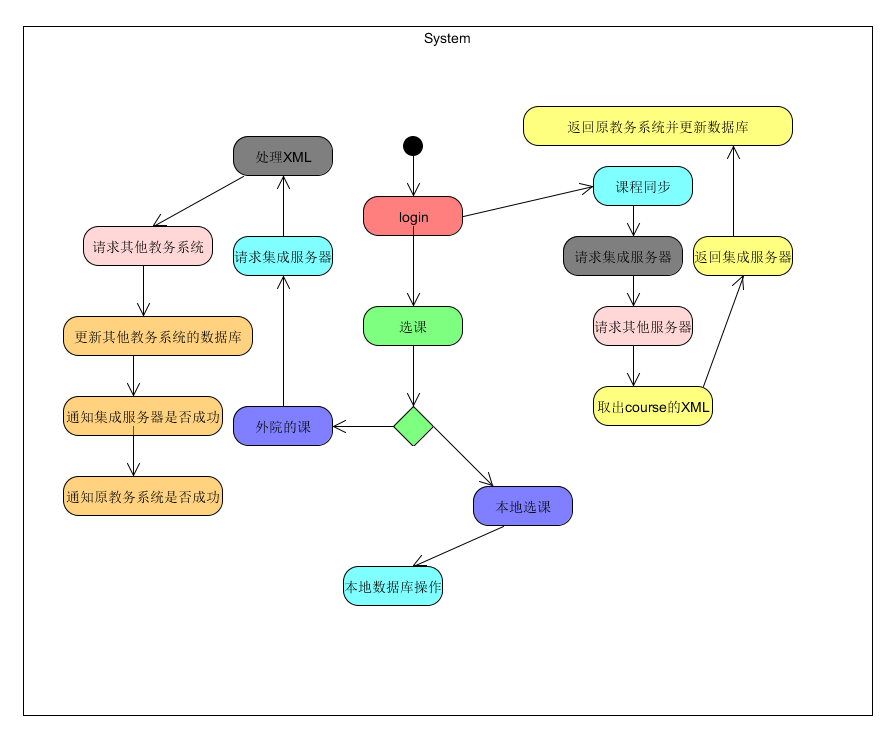
\includegraphics[width=2.4in]{img/1.PNG}
    \caption{Activity Diagram of Integration Homework 1}
  \end{figure}
\end{frame}


\section{Perspectives of Designs}
\begin{frame}
  本次作业的3个关注点:
  \begin{enumerate}
  \item
    可构建性
    \pause
  \item
    统一接口
    \pause
  \item
    通用组件
    \pause
  \end{enumerate}
\end{frame}


\subsection{Buildability}
\begin{frame}
  \begin{enumerate}
  \item
    目标:写完Server\_A后,复制这个项目,然后更改1行代码即可完成Server\_B, Server\_C和Server\_I的部署。
    \pause
  \item
    不同项目的区别在于url不同。需要把这种代码上的变量进行集中控制。
    \pause
  \end{enumerate}
\end{frame}

\begin{frame}
  \begin{figure}
    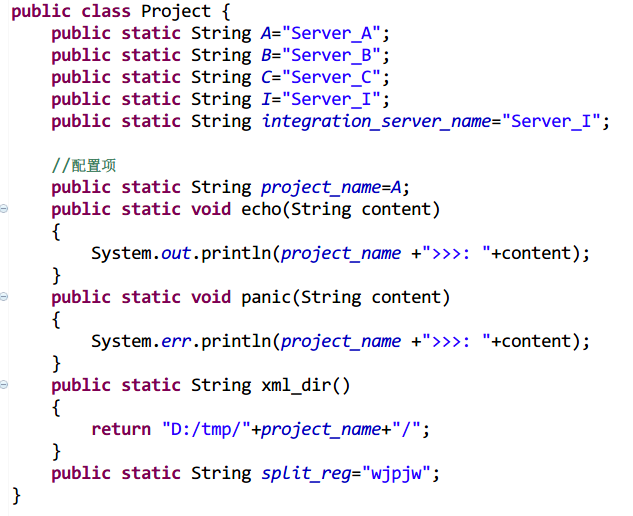
\includegraphics[width=2.4in]{img/2.PNG}
    \caption{Project Config}
  \end{figure}
\end{frame}

\begin{frame}
  \begin{enumerate}
  \item
    我们的项目跨越了多个生态系统。语言上包括Html, JS, JSP, Java, SQL,部署环境包括数据库,服务器端程序,Web客户端。
    \pause
  \item
    我们遇到的一个重要的可构建性问题就是如何进行不同子系统的交互。
    \pause
  \item
    Google有一个protocol buffer就是设计来解决这个问题的,非常不好用。因为Google没有办法让它的标准成为一切的标准。
    \pause
  \item 我们需要一个普世的标准化的可扩展的数据类型能够作为不同系统交互的接口。\pause
  \item 目前软件行业里没有一个保有数据结构的标准数据类型,仅有的通用接口是文本流。\pause
  \item 所以,我们用文本流。\pause
  \item 至于XML,只是文本流的一种协议与规范,在各个平台下都能勉强解析出来,可以用作数据交互。更何况项目中传递的文本流不一定是XML,也可以包括其他信息,所以说我们使用的接口是文本流,而非XML。
  \end{enumerate}
\end{frame}


\subsection{Universal Interface}
\begin{frame}
 \begin{enumerate}
   \item 文本流是通用接口,至今没有什么可行的替代方案。\pause
\item 它有很多缺点,比如说它的耦合是隐式的,这对编程来说带来了挑战,如果多人合作项目的规格没写完善,可能导致很难消除的bug。不过这对于我们来说不是问题,涉及到隐式耦合的地方都直接完成了编码,没有拖延。\pause
\item 文本流的优点是计算机系统的任意子集都必须支持它,唯一比较麻烦的是编码,不过如果数据全是英文的,那么可以不去管编码。\pause
 \end{enumerate}
\end{frame}  
\begin{frame}
 \begin{enumerate}
 \item 一个使用文本流作为通用接口的例子就是SaxParseService这个类。
 \item 这个类用的时候传入的参数全是字符串或者字符串数组。可以做到通用的XML解析,不依赖于model里面的任何模型。
 \end{enumerate}
\end{frame}  


\subsection{Reusable Composites}
\begin{frame}
  为了更好地完成这个项目,我完成了3个独立的模块,与项目本身没有任何耦合。
  \begin{enumerate}
  \item wjp.xml
  \item wjp.fileio
  \item wjp.http
  \end{enumerate}
\end{frame}  


\section{Acknowledgements}

\begin{frame}
\begin{center}
\Huge{Thanks}
\end{center}
\end{frame}


\end{document}


